\documentclass[a4paper,12pt]{article}
\usepackage[utf8]{inputenc}
\usepackage[T1]{fontenc}
\usepackage[polish]{babel}
\usepackage{graphicx}
\usepackage{float}
\usepackage{amsmath}
\usepackage{geometry}
\usepackage{hyperref}
\usepackage{booktabs}

\geometry{margin=2.5cm}

\title{Sprawozdanie: Porównanie implementacji algorytmu Dijkstry}
\author{Marcel Musiałek (Nr Indeksu: 279704)}
\date{27 stycznia 2026}

\begin{document}

\maketitle

\section{Opis implementacji i złożoność obliczeniowa}

W ramach zadania zaimplementowano trzy warianty algorytmu wyznaczania najkrótszych ścieżek w grafie z nieujemnymi wagami krawędzi.

\subsection{Algorytm Dijkstry (Wariant podstawowy)}
Implementacja wykorzystuje standardową bibliotekę C++ (\texttt{STL}). Jako kolejkę priorytetową zastosowano kontener \texttt{std::priority\_queue}, który jest implementacją kopca binarnego.
\begin{itemize}
    \item \textbf{Szczegóły implementacji:} Użyto techniki \textit{lazy deletion} – wierzchołki nie są usuwane z kopca przy aktualizacji odległości, lecz dodawane ponownie z nowym priorytetem. Nieaktualne wpisy są ignorowane przy zdejmowaniu z kolejki.
    \item \textbf{Złożoność obliczeniowa:} Operacje na kopcu binarnym zajmują $O(\log K)$, gdzie $K$ to liczba elementów w kopcu (w najgorszym razie $K \approx m$). Całkowita złożoność wynosi $O(m \log n)$.
\end{itemize}

\subsection{Algorytm Diala}
Jest to implementacja algorytmu Dijkstry wykorzystująca strukturę kubełkową (buckets). Każdy kubełek $k$ przechowuje listę wierzchołków o tymczasowej odległości równej $k$.
\begin{itemize}
    \item \textbf{Szczegóły implementacji:} Ze względu na specyfikę algorytmu, liczba kubełków jest zależna od maksymalnej wagi krawędzi $C$. Algorytm porusza się cyklicznie lub liniowo po kubełkach.
    \item \textbf{Złożoność obliczeniowa:} $O(m + C)$, gdzie $C$ to maksymalny koszt (waga) krawędzi.
    \item \textbf{Ograniczenia:} Algorytm jest bardzo wydajny dla małych wag całkowitych, ale jego złożoność pseudowielomianowa czyni go nieużywalnym dla grafów o dużych wagach (np. rodziny \texttt{Long-C}), gdzie czas wykonania drastycznie rośnie.
\end{itemize}

\subsection{Algorytm Radix Heap}
Zoptymalizowana wersja algorytmu kubełkowego, wykorzystująca własności reprezentacji binarnej liczb. Kubełki przechowują wierzchołki w zakresach odległości $[x, x+2^k)$.
\begin{itemize}
    \item \textbf{Szczegóły implementacji:} Zastosowano funkcję wbudowaną kompilatora GCC \texttt{\_\_builtin\_clzll} (Count Leading Zeros) do błyskawicznego wyznaczania indeksu kubełka w czasie $O(1)$. Zastosowano mechanizm \textit{lazy deletion} oraz bezpieczną redystrybucję elementów z wykorzystaniem \texttt{std::swap} (w celu uniknięcia błędów segmentacji).
    \item \textbf{Złożoność obliczeniowa:} $O(m + n \log C)$.
    \item \textbf{Ograniczenia:} Implementacja jest wrażliwa na przepełnienie zakresów (integer overflow) przy ekstremalnie dużych odległościach skumulowanych (np. w grafach \texttt{Long-n} o dużej średnicy), co może prowadzić do błędów wykonania.
\end{itemize}

\section{Wyniki eksperymentów}

Testy przeprowadzono na komputerze z systemem Linux (CachyOS). Dla każdego testu mierzono średni czas wyznaczenia najkrótszych ścieżek od źródła do wszystkich wierzchołków (tryb SS), uśredniony dla 1 ustalonego i 5 losowych źródeł.

\subsection{Wykresy czasu działania}

\begin{figure}[H]
    \centering
    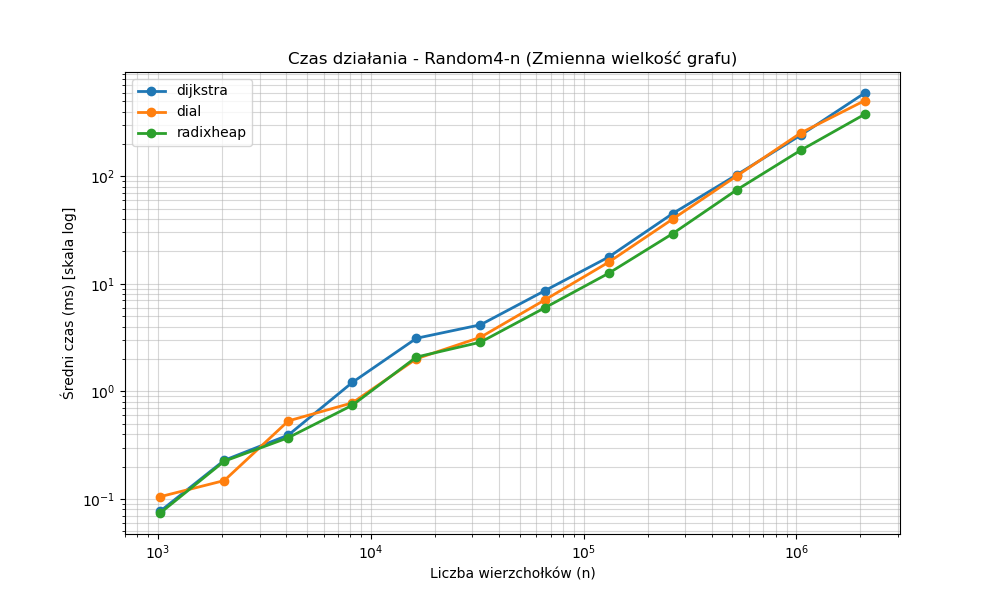
\includegraphics[width=0.8\textwidth]{wykresy/Random4-n.png}
    \caption{Czas działania dla rodziny Random4-n (zmienne $n$).}
\end{figure}

\begin{figure}[H]
    \centering
    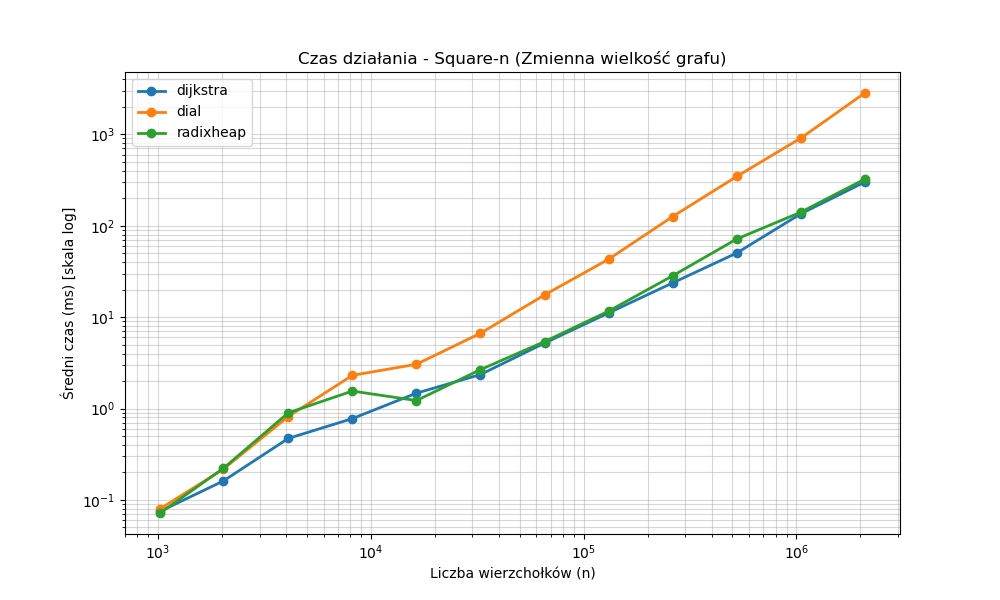
\includegraphics[width=0.8\textwidth]{wykresy/Square-n.png}
    \caption{Czas działania dla rodziny Square-n (zmienne $n$).}
\end{figure}

\begin{figure}[H]
    \centering
    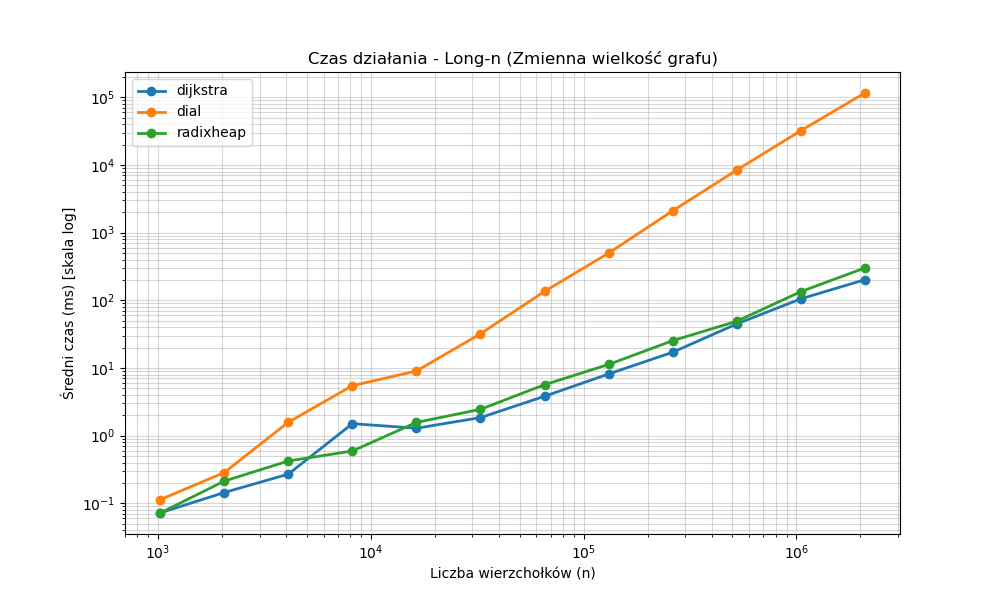
\includegraphics[width=0.8\textwidth]{wykresy/Long-n.png}
    \caption{Czas działania dla rodziny Long-n (zmienne $n$).}
\end{figure}

\begin{figure}[H]
    \centering
    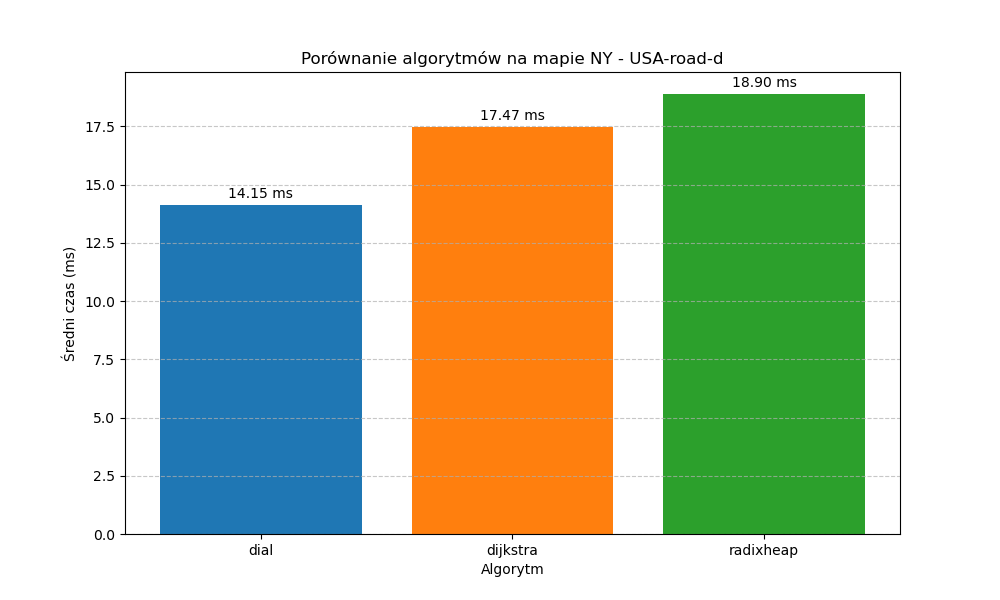
\includegraphics[width=0.8\textwidth]{wykresy/USA-road-d.png}
    \caption{Porównanie algorytmów dla mapy drogowej USA (NY).}
\end{figure}

\begin{figure}[H]
    \centering
    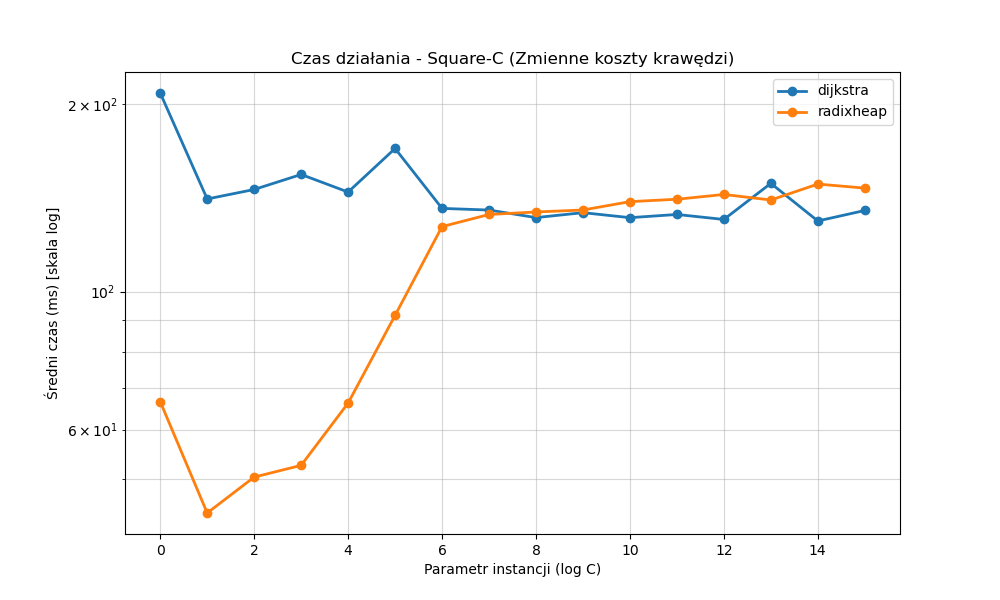
\includegraphics[width=0.8\textwidth]{wykresy/Square-C.png}
    \caption{Czas działania dla rodziny Square-C (zmienne wagi $C$).}
\end{figure}

\subsection{Wyniki P2P dla największych instancji}
Poniższa tabela przedstawia długości najkrótszych ścieżek dla wybranych par wierzchołków w największych badanych grafach.

\begin{table}[H]
    \centering
    \caption{Długości ścieżek (P2P) dla największych instancji.}
    \vspace{0.3cm}
    \begin{tabular}{|l|l|c|r|}
    \hline
    \textbf{Rodzina} & \textbf{Plik} & \textbf{Para (u, v)} & \textbf{Dystans} \\ \hline
    Random4-n & Random4-n.21.0.gr & (1, 2097152) & 9\,051\,281 \\ \hline
    Square-n  & Square-n.21.0.gr  & (1, 2096704) & 714\,640\,488 \\ \hline
    Long-n    & Long-n.21.0.gr    & (1, 2097152) & 31\,336\,751\,771 \\ \hline
    USA-road  & USA-road-d.NY.gr  & (1, 264346)  & 495\,306 \\ \hline
    \end{tabular}
\end{table}

\section{Interpretacja wyników i wnioski}
Analiza przeprowadzonych eksperymentów pozwala na sformułowanie następujących wniosków:

\begin{enumerate}
    \item \textbf{Stabilność algorytmu Dijkstry:} 
    Standardowa implementacja z kopcem binarnym ($O(m \log n)$) okazała się najbardziej uniwersalna. Działała stabilnie dla wszystkich rodzin grafów, niezależnie od struktury czy wielkości wag. Jest to najbezpieczniejszy wybór do ogólnych zastosowań, co widać na wykresach – linia Dijkstry nigdy nie "wystrzeliła" w górę tak gwałtownie jak konkurencja.

    \item \textbf{Niejednorodna wydajność algorytmu Diala:}
    \begin{itemize}
        \item Algorytm "zabłysnął" na rzeczywistej mapie drogowej (USA-road-d), gdzie wyprzedził Dijkstrę (14.15 ms vs 17.47 ms).
        \item Jednak w testach syntetycznych (rodziny Square-n i Long-n), mimo małych wag, algorytm okazał się najwolniejszy. Widać, że algorytm tracił czas na iterowanie po pustych kubełkach, co przy takiej strukturze grafu niweluje jego teoretyczną przewagę. Zysk z braku kopca został "zjedzony" przez konieczność sprawdzania pustych indeksów w tablicy.
        \item Dla dużych wag (rodziny -C) algorytm zgodnie z teorią stał się nieużywalny.
    \end{itemize}

    \item \textbf{Specyfika Radix Heap:}
    \begin{itemize}
        \item Ten algorytm dobrze radził sobie w testach syntetycznych (Square-n), często dorównując lub nieznacznie wyprzedzając Dijkstrę.
        \item Co ciekawe, na mapie USA (Rysunek 4) Radix Heap wypadł najgorzej (18.90 ms). Sugeruje to, że narzut na zarządzanie bardziej skomplikowaną strukturą danych (operacje bitowe, przenoszenie kubełków) nie zawsze zwraca się w praktyce, jeśli graf nie jest specyficznie dopasowany pod ten algorytm.
        \item Podobnie jak w przypadku Diala, przy bardzo dużych odległościach (Long-n) pojawiły się problemy z przekroczeniem zakresów zmiennych (overflow).
    \end{itemize}

    \item \textbf{Wpływ topologii:} 
    Struktura grafu ma kluczowe znaczenie. Algorytmy kubełkowe (Dial) zyskały przewagę jedynie na gęstej siatce mapy drogowej. Na rzadszych grafach syntetycznych ich wydajność spadała, przez co standardowy Dijkstra okazał się "złotym środkiem" – może nie zawsze najszybszym, ale najbardziej przewidywalnym.
\end{enumerate}

\end{document}